\section{Introduction}
Time-series anomaly benchmarks repeatedly join stored detector scores with
labels to evaluate and compare models. A range-aware metric can require a
complete pass through the same series at every score threshold, and a volume
metric repeats this work across temporal widths. Sampling the thresholds
reduces work but changes the numerical query. Our question is which local
statistics suffice to answer the original query exactly.

We study two established operators. Dynamic Volume Under the Surface
(VUS) integrates precision--recall (PR) or receiver-operating-characteristic
(ROC) curves over temporal widths~\cite{paparrizos2022,boniol2025}. Tatbul range
precision and recall reward positional overlap and penalize fragmentation of
true and predicted intervals~\cite{tatbul2018}. Both are used in public
evaluation software. TimeEval's maintainers explicitly identify slow range
metrics and threshold sampling as an optimization opportunity~\cite{timeevalrangeissue}.
These operators have different state dependencies: VUS can omit inactive
support events, whereas range precision changes even when a point outside
every true interval joins two predicted components.

Consider the four-point example $y=(1,0,1,0)$ and $s=(3,2,1,0)$.
Removing off-label events and connecting the remaining ROC endpoints changes
zero-width VUS-ROC from .625 to .8125. An omitted run must instead contribute
its predecessor rectangle. For range metrics, dropping an off-label point can
change predicted intervals and therefore their precision denominators. The
same intuitive ``ignore irrelevant points'' shortcut cannot serve both
operators. We derive the sufficient state for each.

For VUS, complete global ties, predecessor rectangles and two-distance
interval geometry give a support-sensitive representation. For range metrics,
endpoint activations update one recall contribution and at most three precision
contributions. Fixed-label moment prefixes support moving positional weights,
including a middle bias whose interval midpoint changes after a merge. A
finite-feature theorem covers endpoint-dependent piecewise weights; the
implementation provides four canonical biases and three cardinality factors.
Known query grids can use ordinary offline bucketing instead of sorting every
score. The new result is the metric-specific coupled state, rather than
sorting, prefix sums, caching, or component trees.

The data-management setting is repeated analytics over stored score columns.
We provide complete-call and read-to-result-write experiments, including a
native public TimeEval consumer, and compare with same-compiler conventional
controls. We do not propose a detector, a new accuracy metric, an unlabeled
model selector, or a database engine. Our earlier public Sparse VUS 0.3.0
release~\cite{sparsevus03} is an unrefereed software precursor; its speed is
separated from subsequent shared-label computation. It contains no weighted
range trajectory implementation.

The contributions are: (i) exact support-event identities for dynamic VUS and
a general local-update theorem for weighted range trajectories; (ii) algorithms
and ablations separating these identities from compilation and work sharing;
and (iii) source-bound evaluation on public data, including a separately
selected panel with unchanged public detectors and native consumer execution.
We retain reused recordings, low-cardinality losses, non-beneficial alternatives,
and consumers whose other metrics dominate total cost.

\section{Target and exact event representation}
For VUS, let $y\in\{0,1\}^n$ contain both classes and $s\in\mathbb{R}^n$ contain finite
scores after binary64 conversion. Larger scores indicate greater anomaly
evidence. Let $P_0=\sum_i y_i$, and let the $K$ maximal original anomaly
intervals have inclusive endpoints $[a_k,b_k]$ in temporal order. Widths are
the integers $w=0,\ldots,L$. The continuous label $a_i^{(w)}$ is one on
original positives. An interval contributes $\sqrt{1-d/w}$ outside its
endpoints at integer distance $1\le d\le\lfloor w/2\rfloor$; contributions
are summed and clipped at one. At $w=0$ no ramp is added. Expanded intervals
that overlap merge, while adjacent nonoverlapping intervals remain separate.
This is the original dynamic VUS target pinned to the official
\texttt{RangeAUC\_volume\_opt} source at revision
\texttt{467bace0}, configured for exhaustive thresholds~\cite{vusreference}.
It is not shared by all software named VUS.

For a threshold $t$, define
\begin{align}
 p_i(t)&=\ind\{s_i\ge t\}, & C(t)&=\sum_i p_i(t),\\
 A(t)&=\sum_i y_i p_i(t), &
 B(t)&=\sum_i(1-y_i)a_i^{(w)}p_i(t),\\
 T(t)&=A(t)+B(t), & P(t)&=P_0+B(t)/2,\\
 N(t)&=n-P(t).
\end{align}
Let $H(t)$ count expanded components hit by at least one predicted positive,
and let $K_w$ count those components. The curve coordinates are
\begin{align}
 R(t)&=\min\{T(t)/P(t),1\}\,H(t)/K_w,\\
 F(t)&=(C(t)-T(t))/N(t), & \pi(t)&=T(t)/C(t).
\end{align}
Precision is used only at nonempty retained thresholds, where $C(t)>0$;
the initial origin requires no precision value.
The denominator is positive: $P(t)\le(n+P_0)/2<n$. ROC integrates trapezoids
from the origin through complete distinct descending score thresholds to
the explicit terminal $(1,1)$. PR uses the right-step sum
$\sum_j(R_j-R_{j-1})\pi_j$, with $R_0=0$. Each VUS scalar is the arithmetic
mean over every width. Signed horizontal ROC increments are preserved; the
derivation does not replace a dynamic denominator by a fixed one.

Let $S_w=\{i:a_i^{(w)}>0\}$, $Q_w=|S_w|$, and $Q=Q_L$. For an active event
with score $v_j$, precompute the complete global counts
$c_j^>=|\{i:s_i>v_j\}|$ and $c_j^\ge=|\{i:s_i\ge v_j\}|$. They include
positions outside $S_w$ and outside $S_L$.

\begin{lemma}[Inactive threshold runs]
Between consecutive active score events at a fixed width, $T,B,P,N,H,R$
are constant. Omitted thresholds contribute a horizontal ROC rectangle and
zero PR area. At an active score, its complete global numerical tie is a
single transition.
\end{lemma}
\begin{proof}
A newly admitted inactive point has zero weight and cannot hit an expanded
component. Only $C$ changes. The horizontal increments
$(\Delta C)/N$ telescope at fixed height $R$. All positions tied with an
active event enter at its global threshold, so both counts must retain them.
\end{proof}

If the previous retained state is $(T_o,N_o,R_o,c_o)$, event $j$ contributes
\begin{align}
 f_j^-&=(c_j^>-T_o)/N_o,\\
 \Delta\mathrm{ROC}_j&=
 (c_j^>-c_o)R_o/N_o+(F_j-f_j^-)(R_j+R_o)/2,\\
 \Delta\mathrm{PR}_j&=(R_j-R_o)T_j/c_j^\ge.
\end{align}
The initial state is $(0,n-P_0,0,0)$, and afterwards $c_o=c_j^\ge$.
Connecting retained endpoints without the intervening rectangle is
incorrect. For example, $y=(1,0,1,0)$, $s=(3,2,1,0)$ and $L=0$ give ROC
area $0.625$; connecting support endpoints alone gives $0.8125$.

\begin{lemma}[Two-distance geometry]
The weight of a non-original point is determined by its distances $d_1,d_2$
to the nearest two distinct original intervals. It is zero if
$d_1>\lfloor w/2\rfloor$, one if $d_2\le\lfloor w/2\rfloor$, and
$\sqrt{1-d_1/w}$ otherwise.
\end{lemma}
\begin{proof}
Every active ramp has weight at least $1/\sqrt2$. Two contributions therefore
clip to one. If exactly one interval contributes, its distance determines
the weight. Distances to ordered intervals are monotone moving away on each
side, so two neighbors on each side contain the nearest two intervals.
\end{proof}

\begin{theorem}[Support-event evaluation]
\label{thm:support-events}
In a unit-cost model with score comparisons and metric arithmetic, including
square roots, both exhaustive scalar integrals can be computed in
$O(n\log(Q+1)+(L+1)Q)$ time and $O(n+Q)$ auxiliary words.
\end{theorem}
\begin{proof}
Extract original intervals and maximum support in $O(n)$ time. Sort the $Q$
support scores and group equal values. Binary-search all $n$ scores among
these groups to obtain complete global counts $c^>,c^\ge$ without sorting
off-support scores, at cost $O(n\log(Q+1))$. The ordered-interval geometry
can be prepared within this bound. At each width, compute support weights,
component membership, grouped masses and first component-hit events in
$O(Q+K)$ time. A scan of the at most $Q$ event groups integrates the
preceding rectangles, complete tied transitions and terminal ROC tail.
The inactive-run lemma makes this identical to the exhaustive target in
exact metric arithmetic. Stream the width mean using input-, support- and
interval-sized arrays. Since $K\le Q\le n$, the stated bounds follow.
\end{proof}

\begin{proposition}[Fixed-binary64 preparation]
\label{prop:radix}
For finite binary64 scores, complete global tie counts, the score ordering
of maximum support, and its two-distance geometry can be prepared in
$O(n+Q+K)$ time and $O(n+Q)$ auxiliary words. Discrete work uses a word-RAM
with input indices, counts, widths, and intermediate index arithmetic
fitting words. Metric arithmetic, including square roots, has unit cost.
\end{proposition}
\begin{proof}
Normalize signed zeros. Complement a negative score's bit pattern and flip
the sign bit of a nonnegative score, then complement the result to obtain a
descending numerical key. Eight stable byte-counting passes order these
64-bit keys in $O(n)$ time. Scan complete ties and retain their starting and
ending global ranks. Filter the permutation to maximum-support positions.
A temporal scan with a monotone interval pointer computes nearest distances
and owners in $O(Q+K)$ time. All arrays are input- or support-sized.
\end{proof}
Radix sorting and floating-point key transforms are established
techniques~\cite{demaine2011radix,herf2001radix}. This assumption does not give
linear sorting of arbitrary real scores or a bit-complexity bound for growing
precision. Conversion defines numerical ties, including collisions between
distinct large integer inputs.

The same support-event width kernel combined with this preparation gives
$O(n+(L+1)Q)$ time. This is the basic Sparse VUS evaluator; its improvement
over a dense rank sweep depends on $Q$, rather than recall saturation.
The released PR-only implementation retains $L+1$ scalar width results,
adding $O(L)$ words; streaming removes this storage. Input-sized ranking
arrays remain necessary in this construction, so the memory is not
support-only.


\section{Prior VUS algorithms and shared labels}
Boniol et al. already distinguish maximum-buffer support from unaffected
regions and reuse static work~\cite{boniol2025}. Klein's fast-VUS uses
support-score cumulative sums; Benchopt uses dense cumulative sums and segment
maxima~\cite{klein2026,benchopt2026}. Their public exact configurations use
$H=n$, rather than the sampled defaults. The inspected Klein implementation
still constructs full-length coverage arrays at each width; Benchopt builds
full-series cumulative sums and returns both ROC and PR. These array operations
are distinct from the support-event representation. We compare equal returned
work separately from the cost of an available PR-only API.

Sylligardos's efficient VUS work and the public FF-VUS implementation are
important acceleration antecedents~\cite{sylligardos2025,ffvus2026}. The latter
uses linear/max ramps differing from our pinned dynamic target, rounds scores
in its wrapper, and has an approximate existence fallback in its Torch path.
We retain source-level semantic witnesses; native FF-VUS timings would not be
equal-output speed ratios. No experiment here establishes superiority over an
unmeasured GPU evaluator. Complete ties and trapezoidal sweeps are established
ROC techniques~\cite{fawcett2006}; full-recall PR stopping is present in
scikit-learn~1.0.2~\cite{sklearn102}. Neither is claimed as new.

For $M$ profiles sharing labels, the \emph{geometry} variant prepares original
intervals, support and distances once. The \emph{stream} variant additionally
interchanges width and model loops: each width's weights and component
identifiers are prepared once, while all model-specific grouped masses and
complete events remain separate. Under Proposition~\ref{prop:radix}, this costs
$O(Mn+(L+1)MQ)$ time. Its retained workspace after conversion and validation is
$O(MQ+n+Q+K)$: two model-by-support rank/count arrays occupy $16MQ$ bytes.
The public NumPy validation and conversion can allocate $M\times n$ arrays,
giving the more conservative peak bound $O(Mn+MQ+n+Q+K)$. Sharing can therefore
use more memory. Caching and loop interchange are standard optimizations; their
increment is measured against the released evaluator.

An earlier active-prefix alternative uses reversible interval updates and
complete-tie recall saturation, with predicate $A+B/2\ge P_0$ and $H=K_w$.
Its conditional bound and a single-interval run variant remain in the artifact.
The default-width prefix route did not pass its runtime target. This outcome
motivates measuring actual visited work rather than assuming early saturation.

\section{Incremental weighted range precision and recall}
\label{sec:weighted-range}
Tatbul range metrics score intervals using positional overlap and
fragmentation~\cite{tatbul2018}. TimeSeAD already evaluates every observed
score threshold~\cite{wagner2023timesead,timeseadclassic}, and TimeEval exposes
weighted range PR curves~\cite{timeevalrangecurve2026}. We address their
repeated recomputation by maintaining both sides of the metric as predicted
intervals appear, extend, and merge.

\paragraph{Target.}
Let $T_j=[a_j,b_j]$, $j=1,\ldots,K$, be the maximal positive intervals of
fixed binary labels $y$. Predictions use $p_i(t)=\ind\{s_i>t\}$, distinct from
the VUS convention. Let $C$ range over current maximal predicted intervals.
For $X\in\{P,R\}$, weights $w_X(i;a,b)\geq0$ depend on the scored interval's
endpoints, with $Z_X(a,b)=\sum_{i=a}^b w_X(i;a,b)>0$. Define
\[
 W_j=\sum_{i\in T_j}p_iw_R(i;a_j,b_j),\qquad
 N(C)=\sum_{i\in C}y_iw_P(i;a,b).
\]
Write $c_j$ for the number of predicted intervals intersecting $T_j$ and
$h(C)$ for the number of true intervals intersecting $C$. For $\alpha\in[0,1]$,
\begin{align}
 r_j&=\alpha\ind\{c_j>0\}
 +(1-\alpha)g_R(c_j,|T_j|)\frac{W_j}{Z_R(a_j,b_j)},\\
 \psi(C)&=g_P(h(C),|C|)\frac{N(C)}{Z_P(a,b)},\\
 R&=\frac1K\sum_jr_j,\qquad
 P_\rho=\frac{\sum_C\rho(C)\psi(C)}{\sum_C\rho(C)}.
\end{align}
Zero-overlap terms and empty averages are zero; factors are never evaluated
at count zero. Effective cardinality factors $g_P,g_R\in[0,1]$ are pure
functions of count, interval length, and fixed configuration. Let
$C_\gamma(n)\geq1$ bound either factor's arithmetic/comparison evaluation cost
for $1\leq c\leq L\leq n$, using $O(1)$ auxiliary arithmetic words.
Canonical factors satisfy $g(1,L)=1$. The positive, endpoint-local aggregation
weight $\rho$ costs constant time: $\rho=1$ gives macro precision and $\rho=|C|$
gives length-weighted precision over \emph{all} predicted intervals.

\paragraph{Weight family.}
For every $[a,b]$, suppose each weight partitions the interval into at most
$q\geq1$ contiguous integer pieces $I_r(a,b)$, on which
\[
 w_X(i;a,b)=\sum_{k=0}^{d-1}\theta_{Xrk}(a,b)\phi_k(i),\qquad d\geq1.
\]
Features are endpoint-independent and their values and prefixes require
$O(dn)$ preprocessing. Piece endpoints and coefficients require $O(qd)$
work per scored interval. These are explicit arithmetic-cost assumptions,
not permission for arbitrary root finding or mask-dependent callbacks.
Piecewise polynomials of degree at most $d-1$ use $\phi_k(i)=i^k$.
Fixed-label prefixes of $y_i\phi_k(i)$ and $\phi_k(i)$ recover $N(C)$ and
$Z_P(C)$ by summing $qd$ coefficient-weighted prefix differences. Recall
weights have fixed endpoints and can be precomputed once.

\begin{theorem}[Joint weighted range trajectory]
Under these assumptions, $H$ arbitrary threshold queries on $n$ points take
\[
 O\bigl(n\log(n+1)+H\log(H+1)+n(qd+C_\gamma(n))+H\bigr)
\]
time and $O(dn+n+H+qd)$ words in a unit-cost model of exact arithmetic and
comparisons. Constant-cost factors recover
$O(n\log(n+1)+\allowbreak H\log(H+1)+\allowbreak qdn+H)$.
The stated coefficient and cardinality evaluation costs are assumptions;
the bound counts arithmetic operations, not exact-rational bit complexity.
\end{theorem}
\begin{proof}
Maintain the active mask, every $(W_j,c_j)$, and the sums defining $R$ and
$P_\rho$. Precompute in $O(n)$ time an owner array mapping each labeled point
to its true interval. For each active component $[a,b]$, store its left boundary at $b$
and its right boundary at $a$; interior entries may be stale. Initially all
statistics are zero.

Inserting $i\in T_j$ adds its fixed weight to $W_j$ and changes
\[
 c_j\leftarrow c_j+1
 -\ind\{i-1\text{ active in }T_j\}
 -\ind\{i+1\text{ active in }T_j\}.
\]
Replace only $r_j$. Restricted to a contiguous true interval, active runs
correspond exactly to intersecting predicted components. An insertion outside
all true intervals cannot connect two fragments inside one such interval,
because their unique path lies inside it. Existence uses $c_j>0$, even when
a detected point has zero weight.

For precision, remove the zero, one, or two adjacent component contributions
and add their replacement interval. An active neighbor of an inactive point
must be an endpoint, so the stored boundaries identify both components in
constant time; stale interior entries are never queried. Update the new
outer endpoints and both precision sums. With $\sigma_i$ indicating a true
interval start and $D(t)=\sum_{i<t}\sigma_i$,
\[
 h([a,b])=D(b+1)-D(a)+y_a-\sigma_a.
\]
Thus each insertion evaluates at most three precision and two recall terms
in $O(qd+C_\gamma(n))$ work
and preserves every invariant. Fixed-weight preprocessing costs at most
$O(qdn)$ using one coefficient list as scratch. Sort scores and queries
descending, activate all points strictly above each query, and emit only
after complete ties. Each point activates once; output restoration costs
$O(H)$. The prefix tables, maintained state, scratch, and outputs give the
space bound.
\end{proof}

\begin{corollary}[Comparison cost of the complete trajectory]
For constant $q,d$, $C_\gamma(n)=O(\log(n+1))$ and $H=n$, the trajectory takes
$O(n\log(n+1))$ operations. This is worst-case comparison-optimal for
arbitrary distinct real scores and query-associated exact outputs, already
with flat weights and cardinality one.
\end{corollary}
\begin{proof}
Use $n-1$ consecutive positive labels with arbitrary distinct positive scores,
followed by one negative label of score zero; take flat weights, cardinality
one and $\alpha=0$. Request $t_i=s_i$ in input order and write $J$ for the
positive positions. For $i\in J$,
$R(t_i)=|\{j\in J:s_j>s_i\}|/(n-1)$ reveals its rank. A comparison-based
algorithm distinguishes $(n-1)!$ orders and needs $\Omega(n\log n)$ comparisons.
This is the standard sorting reduction. An anonymous multiset of recalls
would not identify ranks. The result concerns full query-associated curves,
not just their maximum, unrestricted algebraic operations, or fixed-width
radix algorithms.
\end{proof}

\paragraph{Constructive relation to a component tree.}
A one-mask Tatbul evaluator can traverse ordered true and predicted intervals
in linear time and compute each positional overlap in closed form; it need
not enumerate every pair of intervals~\cite{tatbul2018}. Our fused raster
avoids all-pairs overlap enumeration but still evaluates point weights. The
separate conventional interval control uses closed-form overlap and fixed-label
prefixes at each query, without cross-threshold state. A classical
threshold component tree additionally supplies births, extensions, merges,
endpoints and component sizes across thresholds~\cite{najman2006,menotti2007}.
Size-based precision/recall through such a tree also predates this
work~\cite{ranefall2016}. These quantities alone do not specify the Tatbul
trajectory: identical scores with different labels give the same tree but
different overlap and fragmentation statistics.

The required augmentation is explicit. Precision uses the true-start prefix
$D$, label-weight prefixes, and the two global sums
$\sum_C\rho(C)\psi(C)$ and $\sum_C\rho(C)$. Recall additionally needs one
$(W_j,c_j)$ pair per true interval and $\sum_j r_j$. At each activation:
\begin{quote}\small
Remove the precision terms of adjacent active components.\\
If $i\in T_j$, replace $r_j$ using the updated $W_j,c_j$.\\
Join the adjacent components through $i$; update the outer endpoints.\\
Compute the replacement component's $h,N,Z,\rho$ from the prefixes and
add its precision term.\\
After the complete eligible tie or query bucket, emit the two global averages.
\end{quote}
An explicit component tree augmented with these identities is an alternative
implementation of the same algorithmic class. The endpoint representation
avoids materializing a hierarchy that these queries do not consume; we claim
no asymptotic superiority over that augmented tree. The metric-specific
contribution is the coupled sufficient state and its local identities.

Moving weights require more than a single component count and moment. On
positions $0,1,2,3$, label patterns $1001$ and $0110$ both have count two and
first moment three, yet middle-weight masses two and four. Prefix queries on
the two sides of the current midpoint recover this distinction after every
merge without revisiting the component's points.

An off-label bridge can change precision even though every recall contribution
is unchanged. With $y=(1,1,0,0,1,1)$ and $p=(0,1,1,0,1,1)$, reciprocal
cardinality and middle precision bias give macro precision
$(1/2+1)/2=3/4$. Activating zero-based index 3 joins $[1,2]$ and $[4,5]$ into
$[1,5]$: its weight mass is 4 of 9 and it intersects two true intervals, so
precision becomes $(1/2)(4/9)=2/9$. The fixed true intervals retain their
overlap and fragmentation. This is why off-label activations and moving
normalizers must both participate in the precision update.

\paragraph{Finite query grids and consumers.}
Full score sorting is unnecessary for a known grid. Binary-search each
score's first strictly eligible query among descending thresholds, then
counting-bucket its activation. Processing complete buckets preserves the
queried masks regardless of internal order, giving
\[
 O\bigl(n\log(H+1)+H\log(H+1)+n(qd+C_\gamma(n))+H\bigr).
\]
Already ordered queries omit their sorting cost. A consumer that subsequently
sorts by recall, such as TimeEval, adds $O(H\log(H+1))$; its endpoints and
integration convention remain part of its contract. Range recall need not
be monotone. Strict observed-score queries exclude the all-active state
below the minimum; include a lower sentinel when required.

\paragraph{Implemented family.}
For $u=i-a+1$ and $L=b-a+1$, the canonical choices are
\[
\begin{array}{c|c|c}
\text{bias}&w(u,L)&Z(L)\\\hline
\text{flat}&1&L\\
\text{front}&L+1-u&L(L+1)/2\\
\text{back}&u&L(L+1)/2\\
\text{middle}&\min(u,L+1-u)&\lfloor(L+1)^2/4\rfloor
\end{array}
\]
They need at most two pieces and first moments. Middle precision queries
both sides of the moving midpoint; an unsplit count and moment are
insufficient. Precision and recall biases are independently selectable.
Implemented cardinalities are $1$, $1/c$, and TimeSeAD's
$((L-1)/L)^{c-1}$, with value one at $c=1$~\cite{wagner2023timesead}.
The first two require $O(1)$ exact arithmetic operations; repeated squaring
evaluates the third in $O(\log(n+1))$ operations with $O(1)$ arithmetic registers.
Thus all three retain the complete-trajectory bound, whereas the grid's
linear update term requires constant-cost factors or fixed-format evaluation.
One shared cardinality choice and macro or length-weighted precision are
implemented. Separate generic callbacks, polynomial weights, and the broader
finite-feature interface are theorem-only generalizations.

\paragraph{Numerical scope and antecedents.}
Integer counts and first moments avoid cancellation from subtracting rounded
floating prefixes. For the canonical family, $n\leq2^{31}-1$ bounds all
intermediate products within signed int64; this restriction does not certify
higher-degree polynomials. The improved factor uses a count-one branch and
$\exp((c-1)\operatorname{log1p}(-1/L))$. Division and accumulated differences
still round: real-arithmetic equality is neither bitwise agreement nor a
length-independent floating-point certificate. Scores are finite binary64;
query infinities provide sentinels, and ties are complete.

Tatbul already gives closed-form overlap evaluation~\cite{tatbul2018}.
Component trees and attribute maintenance are classical~\cite{najman2006};
Menotti et al. give linear-time 1D construction with height, surface, and
volume attributes~\cite{menotti2007}. We claim neither new positional biases
nor a new component tree. The contribution is the coupled, label-conditioned
overlap and fragmentation state across thresholds; ordering and bucketing
are standard offline techniques.


\section{Experimental design}
\label{sec:design}
We distinguish the original VUS/range panel, a separately selected weighted
panel, and native consumer queries. Each follow-up freezes its own methods,
inputs, orders and censoring rule before its measurements; it is not a
retrospective enlargement of the original protocol. All exact comparisons
hold the metric definition and query set fixed. Comparing sampled and complete
queries is instead an accuracy--cost analysis.
The study-to-output map is: dynamic VUS returns integrated ROC/PR values
(primary VUS-PR comparison in Table~\ref{tab:vus-main}); flat and weighted range
studies return strict-query precision/recall/F1 trajectories and maximum F1
(Tables~\ref{tab:range-main},~\ref{tab:weighted-new},~\ref{tab:interval-control});
native TimeEval returns three integrated metrics, with inclusive range queries
and synthetic endpoints (Tables~\ref{tab:native-mac},~\ref{tab:native-linux}
and~\ref{tab:native-control}; process-session follow-up in
Table~\ref{tab:affinity-blocks}).
These contracts are compared internally, not treated as interchangeable outputs.
An initial weighted Mac run was stopped after 12 WSD cases and one Stock
query contract. Before a complete rerun, we separated paired-order timing
uncertainty from recording sensitivity and bound the independent auditor in
the protocol. Cohort, profiles, semantics, methods, orders and hypotheses were
unchanged. The 5,400 partial records are retained but excluded from the final
study; its analysis protocol was therefore fixed after this partial pilot,
not before every observation in the research process.

\paragraph{Original panel and its dependence.}
The pinned TSB-AD-U archive~\cite{tsbad} supplies all eligible NAB, SMAP and SMD
recordings after six named development exclusions, source-labelled synthetic
exclusions and exact observation-plus-label deduplication. The 73 recordings
(20/17/36 by collection) have lengths 1,000--28,696. Eight fixed CPU procedures
produce Isolation Forest, LOF, nearest-neighbor, one-class SVM, PCA, KMeans,
HBOS and shrinkage-Mahalanobis scores. They use trailing length-16 windows,
an evenly spaced unlabeled fit set capped at 2,048 points, and seed 20261024.
These authored offline transductive procedures are workload generators, not
reproductions of eight tuned benchmark pipelines. LOF novelty-mode scoring
includes fit points. All 584 outputs retain binary64 scores without jitter or
rounding; distinct counts range from 3 to 28,696. A five-distinct-cluster warning
for requested 16-cluster KMeans remains in the record.

Sixty-two recordings were used by name in older repository studies. SMD's
36 cases have nine distinct label sequences; 18 share labels with excluded
development recordings. We report label-block weighting and exclusion
sensitivity. These checks do not establish independent physical sources, and
fresh scores do not make the recordings unseen.

\paragraph{Separately selected public-detector panel.}
Before fitting or metric outcomes, we screen archive candidates against 563
prior provenance entries by name, exact labels, exact observations, and
z-normalized observations rounded to ten decimals. We select 12 WSD recordings
at fixed length quantiles among 91 eligible cases, all 12 eligible Stock cases,
and both eligible MSL cases. The 26 recordings contain 386,447 observations.
This screening removes the declared forms of reuse; it cannot prove absence
of shifted variants or common physical sources. In particular, MSL is only two
recordings, not a broad new-domain sample.

Unchanged public FFT and COPOD APIs at TSB-AD revision \texttt{ed74348e}
generate two profiles per recording, using the full univariate input and their
upstream preprocessing. We perform no extra quantization or model selection.
The fixed seed is 20261024, one thread is used, and the per-fit limit is 120
seconds. All 52 fits complete, with no replacement or retry. A path-packaging
error occurred after the original Mac fits; the receipt was recovered from
their immutable outputs with zero repeated fits. Original producer and recovery
sources are archived. The Linux replay uses the corrected packaging path and
regenerates every score from raw inputs. Following a failed input-identity
check, a separate decoding contract was frozen before fresh Linux fits. It
restores one original Mac binary64 observation that the Linux parsers round
one ULP differently. Its raw-file digest, decimal token, row index, adjacent
binary64 values, and full before/after array hashes are explicit. All original
input-identity checks remain mandatory; this reproduces the frozen typed
input rather than asserting cross-platform identity of the original parser.

\paragraph{Comparators and contracts.}
VUS compares stream, geometry-only, released sparse radix, active prefix,
matched dense radix, unchanged Klein, and a separately frozen Benchopt pair.
An author-created conventional support control shares validation, radix
ordering and global counts, but uses direct per-width ramps instead of nearest
geometry. A minimal Klein ablation changes only its threshold list to distinct
maximum-support scores. These controls isolate compiler, support and sharing
effects; neither is an unchanged public release.

The original flat/reciprocal range study compares vectorized prefix/interval
recomputation, fused compiled raster, score-sorted sweep, and query buckets at
100 evenly spaced strict thresholds. The exhaustive contract evaluates every
observed score under $s_i>t$. It excludes the all-active state below the minimum.
The weighted follow-up uses raster, sweep and bucket with all 12 combinations
of four equal precision/recall biases and three cardinality factors, macro
precision, and recall $\alpha=.2$. Mixed biases and length-weighted precision
are correctness cases, not extra timed workloads. The same compiler and
arithmetic formulas are used for the raster and incremental methods.

A subsequent comparator audit identified an additional conventional control:
Tatbul's closed-form ordered-interval traversal. In a separate frozen ablation,
we precompute fixed-label count/moment prefixes, discover all predicted
intervals by a complete score scan at each query, and compute recall from
ordered intersections and closed-form positional sums. No metric state is
reused across thresholds. Six permutations remeasure raster, this interval
control, and the incremental backend (bucket for grid100, sweep for distinct)
on the unchanged full panel and all 12 semantic choices. This prospective
follow-up isolates conventional per-query optimization from joint state
maintenance; it does not replace the original frozen raster results.

\paragraph{Native TimeEval consumer.}
We pin the complete TimeEval source at \texttt{7c362275}, instantiate its
unchanged \texttt{MetricComputor}, and request ROC-AUC, PR-AUC and range PR-AUC.
The range configuration is \texttt{DefaultMetrics.RANGE\_PR\_AUC}, whose
parameters differ from the range-curve class constructor defaults.
The native loader reads dataset labels and stored scores, computes all three
metrics and writes its result CSV. Only the inner range curve callback is
replaced. Validation, score sanitization, constants, threshold selection,
synthetic endpoints, recall/precision ordering and trapezoidal integration
remain native. This experiment uses flat bias, cardinality one, and zero
existence reward, matching the native default. Its $\ge$ query is mapped to
the strict kernel using the preceding representable binary64 threshold.
It is a different query contract from the strict observed-score F1 study.

We compare the unchanged public callback, compiled raster, and buckets in
two contracts: native nominal \texttt{max\_samples=50}, and every nonminimum
observed-score query, retaining the native synthetic endpoints.
Nominal 50 is not a hard cap: the Mac inputs produce 2--90 actual
queries per profile. The consumer preserves that behavior. Batches are all 52
profiles together and each of the three collections separately. Six method
permutations balance order, giving 144 scheduled trials. A workflow is censored
at 600 seconds; after its first censor, the five remaining same-method/contract/
batch repetitions are explicitly not run. Censored calls provide no completed
public-output parity claim or ordinary timing confidence interval.

\paragraph{Timing and uncertainty.}
Warm operator calls include validation, preparation, sorting, allocation,
curve production and numerical model selection. Whole-consumer clocks include
CSV loading, all three metrics and result-CSV write/close; they exclude imports,
JIT warm-up, trial-directory preparation and audits. Detector fitting, cold
storage and \texttt{fsync} are outside the claimed workload. A sum of case medians
is not described as directly timed collection latency. Numerical libraries use
one thread, but shared-host load is not controlled.

Original VUS case medians use 12 balanced orders, range-grid medians eight, and
the original exhaustive range comparison two AB/BA calls per method. Paired
case log ratios are bootstrapped 10,000 times, with a three-collection Bonferroni
95\% interval per comparator. Label-block sensitivity addresses repeated SMD
geometry. These are fixed-panel sensitivity analyses, not estimates from an
independent random population of recordings.

For the new weighted panel, each case/contract/semantics combination uses six
method permutations. Primary uncertainty resamples paired order indices within
each recording, sharing indices across both methods and all 12 semantics,
recomputes medians, then averages log ratios equally across semantics and
recordings. It is conditional timing uncertainty on the fixed panel. A separate
recording-reweighting bootstrap shows workload sensitivity, especially for
two-recording MSL. Aggregate intervals adjust over three collections; individual
semantics intervals adjust over 36 collection/semantics cells per comparison.
The extreme adjusted quantiles of 10,000 draws are approximate. No host pooling
or favorable-host selection is used. The original and supplemental native
consumer intervals resample six paired complete-workflow trials only when all
six are observed. The separate five-process follow-up instead resamples
process-level mean log ratios, as specified in Table~\ref{tab:affinity-blocks}.

\paragraph{Correctness and selection.}
Complete canonical range curves are archived, including precision, recall and
F1; repeated-output hashes must agree. Independent record auditors import no
metric producer and reconstruct coverage, curve discrepancies, winner sets,
regret and intervals. Finite-set rational oracles additionally cover exhaustive
small tied inputs, with randomized boundary and mixed-weight cases. Public
implementations and a long-window high-precision check provide further
differential evidence. Real-arithmetic identities, empirical binary64 agreement
and a formal rounding certificate are distinct.

Winner sets contain values within $10^{-10}$ of the maximum. Approximation
regret is the best exhaustive value minus the selected model's exhaustive
optimum. The original panel retains minimum and maximum over tied winners;
the weighted panel's prespecified primary statistic uses the best tied winner.
Worst-tie sensitivity is a separate subsequent reconstruction. The predeclared
practical cutoff is .01. This is labeled oracle evaluation, not a deployable
threshold policy or an improvement in detector accuracy.

\section{VUS and original range results}
\begin{table*}[t]\centering\small
\begin{tabular}{lrlll}\toprule
Collection & Cases & Released / stream & Matched dense / stream & Klein exact / stream\\\midrule
NAB & 20 & 1.496 [1.428,1.566] & 3.543 [3.338,3.713] & 30.513 [27.399,33.652]\\
SMAP & 17 & 1.271 [1.242,1.302] & 3.693 [3.196,4.191] & 25.772 [22.941,28.940]\\
SMD & 36 & 1.207 [1.193,1.221] & 3.956 [3.736,4.125] & 25.172 [23.475,26.695]\\
\bottomrule\end{tabular}
\caption{Original VUS complete-call geometric ratios, Apple M1 Pro, width 30,
eight profiles per case. Brackets are 95\% paired-case bootstrap bounds adjusted
over three collections per comparator. They characterize the fixed panel;
source and label dependence remain. All calls include validation, preparation
and winner selection. This is the whole evaluator versus its released
precursor, a matched compiled dense control, and the unchanged public exact API.}
\label{tab:vus-main}\end{table*}

\begin{table*}[t]\centering\small
\begin{tabular}{lrrr}\toprule
Host / collection & Grid100 raster/bucket & Distinct raster/sweep & Distinct wins/cases\\\midrule
Apple NAB & 1.719 [1.625,1.814] & 27.80 [18.74,41.94] & 20/20\\
Apple SMAP & 1.994 [1.817,2.252] & 21.44 [8.57,43.14] & 16/17\\
Apple SMD & 1.969 [1.884,2.095] & 128.08 [95.09,154.61] & 36/36\\\midrule
Linux NAB & 1.900 [1.616,2.239] & 29.35 [18.81,46.08] & 20/20\\
Linux SMAP & 2.898 [2.624,3.260] & 27.76 [11.63,53.75] & 16/17\\
Linux SMD & 3.574 [3.412,3.789] & 163.60 [125.92,193.02] & 36/36\\
\bottomrule\end{tabular}
\caption{Original flat/reciprocal range-F1 study on the same 73 recordings and
584 profiles. Ratios compare identical query contracts against a fused compiled
raster. Familywise 95\% intervals adjust over three collections separately per
comparison. Linux is the selected fresh combined EPYC 7763 execution; generated
scores differ and hosts are not pooled. The exhaustive low-cardinality loss is
retained on both hosts.}
\label{tab:range-main}\end{table*}

\paragraph{VUS attribution.}
At width 30, the whole stream evaluator improves over exact Klein by
25.17--30.51 times geometrically and over a matched compiled dense evaluator
by 3.54--3.96 times (Table~\ref{tab:vus-main}). The public-library advantage
therefore includes implementation effects but is not entirely explained by
them. Independent-call dense/released ratios are 2.37/2.91/3.28. All primary
exact PR calls agree within $1.11\cdot10^{-15}$; matched ROC workflow differences
are at most $4.86\cdot10^{-14}$. Against unchanged Benchopt with equal ROC+PR
outputs, directly timed workflow ratios are 25.3/32.1/40.9.

The new sharing increment is smaller: released/stream ratios are
1.496/1.271/1.207. Geometry reuse already explains most of it on SMAP/SMD;
the additional stream/geometry improvement is 1.094/1.024/1.025, with five
SMAP/SMD case losses. The conventional compiled support control is faster than
the released single-model evaluator on every primary case (ratios
.910/.960/.978, adjusted intervals below one). Thus this panel does not
establish a separate runtime advantage of nearest geometry over optimized
direct ramps. Control/stream ratios remain 1.357/1.201/1.166, including shared
work. The minimal Klein patch alone improves public Klein by 1.65/2.27/2.97;
the remaining released/patch advantage combines additional reductions and
implementation differences. These ablations preclude assigning the entire
public-library gap to one geometric lemma.

At 250 sampled Klein thresholds, 14/73 winner sets change and four have regret
at least .01 (maximum .0584); at 1,000, three change and none has regret .01.
NAB has no changes. Complete stream workflows are nevertheless 7.27--11.25
times faster than the sampled 250-query public API. This comparison has
different outputs and establishes an observed cost/fidelity tradeoff, not
same-query dominance over every approximate algorithm.

\paragraph{Failure regimes and broader VUS checks.}
Primary support fractions are .00384--.223. In a controlled dense-positive
case, dense/released is .980 with interval [.962,.9994]: sparse compression
loses. A one-million-point random-score case visits 99.94\% of support in the
active-prefix algorithm, explaining why saturation is not a general solution.
With one profile, sharing gains only 1.023 times. A six-series development
certificate-plus-fallback route took 33.93 times the direct exact cost and
certified no early selections; this failed route was not promoted.

Eight MITDB and one SWaT recording extend real lengths to 419,919--650,000.
Complete Klein/stream workflow median ratios are 23.10 and 17.70; incremental
released/stream paired intervals [.925,1.340] and [.955,1.165] include one.
These reused follow-up recordings support the whole evaluator more strongly
than the batch refinement. At $n=500{,}000$, eight profiles and positive fraction
.5, process peak RSS is 225.0 MiB for stream, versus released 175.2 and dense
210.6 MiB; lifetime process peaks include libraries, inputs and warm-up.

The earlier unchanged TSB-AD nine-metric consumer shows an Amdahl limit. On
the length-selected SMD case with eight profiles, replacing only VUS reduces
its stage from .9289 to .01406 seconds but total read-to-CSV time from 34.260
to 33.234 seconds: $1.031\times$. All nine outputs agree within
$3.45\cdot10^{-15}$. Two complete repetitions per backend give descriptive
timing, not a population interval. Affiliation and other stages dominate.
The new three-metric TimeEval experiment is a separately defined consumer,
not a revision of this unfavorable observation.

\paragraph{Original flat/reciprocal range trajectory.}
Table~\ref{tab:range-main} compares exhaustive observed-threshold evaluation
against a fused compiled raster, including preparation and winner selection.
The maximum curve difference is $3.00\cdot10^{-15}$, with no method-induced
winner disagreement. Bucketing wins every grid100 case median; the exhaustive
sweep loses on SMAP534, whose eight profiles have only 3--11 distinct values.
Its original Apple raster/sweep ratio is .417, and its fresh Linux ratio .661.
Repeated scanning is competitive when there are very few queries.

Replacing grid100 by complete strict observed thresholds changes 24/73 winner
sets, with 15 disjoint sets and 12 best-selected-model regrets at least .01.
Maximum Apple regrets are .439/.150/.127. These are consequences within a
reused panel of eight authored score procedures. They do not establish a
general prevalence of harmful approximation. Complete sweep costs
2.19/2.14/3.01 times the fastest grid100 bucket method on the original host;
the extra fidelity is not free.

Length-selected public comparisons use the three shortest cases per collection,
all eight profiles, and a declared 60-second per-call budget. TSB-AD grid-F1
values agree within $6.67\cdot10^{-16}$; completed TimeSeAD calls agree within
$5.66\cdot10^{-8}$ under its float32 storage and separate $\alpha=0$ contract.
Two public SMD187 calls are censored and are not counted as parity successes.
All 1,168 unchanged-public binary range-F1 checks at selected cuts agree within
$4.62\cdot10^{-16}$; this validates chosen-cut values, not independent global
maximality. Three million-point stress cases have maximum cross-method curve
error $2.23\cdot10^{-12}$, below the frozen $10^{-9}$ stress tolerance.

\paragraph{Fresh original-panel execution.}
A complete raw-data-to-table replay on an AMD EPYC 7763 independently
regenerates profiles and reproduces the direction of the VUS and range results.
Original VUS released/stream ratios are 1.886/1.580/1.340 and Klein workflow
ratios 20.06/20.28/16.17. The combined range replay retains all generated
arrays and curves, and its four independent reports reconstruct identically.
All 73 score matrices differ bitwise from the Mac; differences are not
uniformly small. The range selection counts remain 24/15/12, but two SMD
recordings exchange flags and maximum SMD regret becomes .0797. A separate SVM
diagnostic finds 104 versus 105 fitted support vectors despite identical raw
and standardized inputs; it does not identify a specific instruction-level
cause. Fresh generation is therefore not an isolated CPU intervention.

\section{Weighted and native consumer results}
\paragraph{Generalized operator on separately selected recordings.}
The completed Mac study contains all 26 recordings, both public detector
profiles, 12 bias/cardinality combinations, both query contracts and all
scheduled methods. The independent reconstruction finds maximum curve
discrepancy $2.50\cdot10^{-15}$ and no same-contract winner disagreement.
Table~\ref{tab:weighted-new} reports equal-semantic-weight geometric ratios
against the fused compiled controls. Grid bucketing improves every recording's
aggregate on all three collections. Exhaustive sweep improves all WSD and
Stock aggregates but only one of two MSL recordings. MSL's exhaustive ratios
are .558 and 3.438, so its narrow paired-timing interval around the aggregate
does not indicate robust benefit across new MSL recordings. The separate
recording-reweighting interval [.558,3.438] exposes this sensitivity.
The 12 individual semantic contracts retain the same collection-level
direction: their exhaustive ratios span 8.388--8.959 (WSD), 20.988--23.321
(Stock), and 1.313--1.449 (MSL). Their grid ratios span 1.506--1.549,
1.472--1.714, and 1.519--1.592, respectively. All adjusted paired-order
intervals for these aggregate semantic cells lie above one. Nevertheless,
every MSL exhaustive contract loses on the same one of its two recordings;
the semantic average does not erase that loss. The artifact retains all 36
collection/semantics rows per comparator with both uncertainty summaries.

\begin{table*}[t]\centering\small
\begin{tabular}{llrrr}\toprule
Host & Collection & Grid100 raster/bucket & Distinct raster/sweep & Distinct recording sensitivity\\\midrule
Apple & WSD & 1.526 [1.518,1.530] & 8.801 [8.727,8.837] & [4.896,14.920]\\
Apple & Stock & 1.621 [1.609,1.628] & 22.635 [22.424,22.810] & [17.181,29.800]\\
Apple & MSL & 1.559 [1.542,1.573] & 1.385 [1.362,1.427] & [.558,3.438]\\
Linux & WSD & 2.097 [2.081,2.101] & 7.460 [7.367,7.484] & [4.290,12.454]\\
Linux & Stock & 1.738 [1.734,1.742] & 15.848 [15.628,15.875] & [13.043,19.373]\\
Linux & MSL & 2.072 [2.045,2.090] & 1.670 [1.659,1.682] & [.859,3.244]\\
\bottomrule\end{tabular}
\caption{Original weighted operator study, Apple M1 Pro and fresh Linux replay.
Within each recording,
log ratios are equally weighted across the 12 prespecified bias/cardinality
contracts. Bracketed ratio columns give approximate 95\% paired-order intervals
conditional on this fixed panel, adjusted over three collections. The last
column separately resamples recordings and is workload sensitivity, not a
population confidence interval. WSD and Stock each have 12 recordings; MSL has
two. All ratios compare identical outputs and queries within a row.}
\label{tab:weighted-new}\end{table*}

Sampling has a smaller selection effect on this panel. Only the middle-bias,
cardinality-one contract produces a nonoverlapping grid-versus-exhaustive
winner set, with maximum best-tie regret .001412; no contract produces
best-tie regret .01. A separate post-hoc saved-curve reconstruction finds
singleton grid winners in all 312 case/semantic combinations, so worst-tie
regret is identical on this Mac panel.
Thus the original 15/73 nonoverlap result does not extend as a prevalence
claim to these two unchanged public detectors. The weighted study supports
computational generality while retaining this negative selection result.

\paragraph{Fresh Linux execution.}
The original fresh replay verifies the raw archive,
425 TimeEval source files and all typed inputs, regenerates 52 detector
profiles, and reconstructs both operator and consumer outputs. Compared with
Mac, all 26 label-array hashes agree but 25/52 score hashes differ, all from
COPOD; FFT's 26 score hashes agree. These are independently generated host
workloads, not an isolated CPU intervention. Native query totals are 2,776
at the nominal default on both hosts and 71,749/71,750 at all observed queries
on Mac/Linux. No timing or uncertainty is pooled across hosts.
The Linux weighted study reconstructs all 11,232 records and 156 curves,
with maximum error $2.50\cdot10^{-15}$ and zero same-contract winner
disagreements. Table~\ref{tab:weighted-new} gives its aggregate results.
Linux MSL id7 loses against exhaustive raster (.859) and against grid sweep
(.963); ten of the MSL collection-level grid sweep/bucket semantic intervals
include one. Thus the Mac semantic result is not asserted uniformly across
Linux contracts. All 312 Linux grid winner sets are also singletons; the
largest best/worst-tie regret remains .001412, with none reaching .01.

\paragraph{Native public consumer.}
The Mac execution completes 120 of 144 scheduled records, with four public
600-second censors and 20 prespecified skips. The independent auditor verifies
all completed CSVs and reconstructs maximum scalar discrepancy
$3.33\cdot10^{-16}$. Completed public outputs cover 28/52 profiles in each
contract (MSL and WSD); Stock has compiled-to-compiled agreement only. Matching
family outputs also verify those same profiles in the combined batch, but do
not supply its censored public execution time.

Table~\ref{tab:native-mac} shows absolute whole-workflow medians and matched
compiled comparisons. At all observed queries, the combined raster/bucket
ratio is 2.728 [2.649,2.801], including native loading, three metrics and result
writing. At the nominal default it is 1.017 [.998,1.039], with no supported
advantage over raster. Public-code engineering gains are much larger: completed
WSD public/bucket ratios are 9.598 [9.438,9.774] at the default and
407.099 [398.649,416.713] at all observed queries. These are not all attributable
to the incremental recurrence. The separately frozen interval control below
tests the remaining conventional-algorithm explanation.

\begin{table*}[t]\centering\small
\begin{tabular}{llrrrr}\toprule
Query contract & Batch (profiles) & Public seconds & Raster seconds & Bucket seconds & Raster/bucket [95\% interval]\\\midrule
Nominal 50 & All (52) & censored $>600$ & 1.0848 & 1.0783 & 1.017 [.998,1.039]\\
Nominal 50 & MSL (4) & .08008 & .03177 & .03291 & .860 [.639,1.014]\\
Nominal 50 & Stock (24) & censored $>600$ & .48931 & .48169 & 1.043 [1.013,1.083]\\
Nominal 50 & WSD (24) & 5.22731 & .55475 & .54321 & 1.019 [1.003,1.037]\\
All observed & All (52) & censored $>600$ & 2.94605 & 1.08068 & 2.728 [2.649,2.801]\\
All observed & MSL (4) & .48152 & .03352 & .03038 & 1.088 [1.045,1.136]\\
All observed & Stock (24) & censored $>600$ & 1.86034 & .50496 & 3.557 [3.354,3.715]\\
All observed & WSD (24) & 234.80063 & 1.07523 & .58478 & 1.866 [1.832,1.901]\\
\bottomrule\end{tabular}
\caption{Native TimeEval read-to-result-write execution on Apple M1 Pro.
Absolute times are medians of six completed workflows. Ratios are geometric
means of six matched-order ratios, not ratios of the displayed medians;
intervals are approximate conditional paired-order intervals. Each censored
public key has one timeout and five unrun repetitions, not a completed median
or interval. The native nominal/all-observed contracts emit 2,776/71,749 queries
across 52 profiles; no cross-contract speed ratio is asserted.}
\label{tab:native-mac}\end{table*}

The original fresh Linux replay also completes 120 workflows, with four
600-second public censors and 20 prescribed skips. It verifies public outputs
for the same 28/52 profiles per contract, with maximum discrepancy
$3.33\cdot10^{-16}$. Table~\ref{tab:native-linux} retains all batch results.
The combined exhaustive raster/bucket ratio is 1.932 [1.907,1.946], smaller
than the separately executed conventional-control replay below. Its default
ratio is 1.014 [1.007,1.027], a small benefit that is not consistently supported
by the other runs' intervals. MSL's exhaustive aggregate does not support a
gain; one bucket trial takes .09497 seconds, versus .04342--.04491 for its
other five trials. That observation is retained, not removed as an outlier.

\begin{table*}[t]\centering\small
\begin{tabular}{llrrrr}\toprule
Query contract & Batch (profiles) & Public seconds & Raster seconds & Bucket seconds & Raster/bucket [95\% interval]\\\midrule
Nominal 50 & All (52) & censored $>600$ & 1.58408 & 1.56792 & 1.014 [1.007,1.027]\\
Nominal 50 & MSL (4) & .25969 & .04442 & .04485 & .992 [.986,.9997]\\
Nominal 50 & Stock (24) & censored $>600$ & .71023 & .70782 & 1.020 [1.003,1.046]\\
Nominal 50 & WSD (24) & 14.44195 & .83543 & .82163 & 1.027 [1.015,1.050]\\
All observed & All (52) & censored $>600$ & 3.04217 & 1.56594 & 1.932 [1.907,1.946]\\
All observed & MSL (4) & 1.94251 & .04737 & .04445 & .941 [.730,1.076]\\
All observed & Stock (24) & censored $>600$ & 1.68294 & .70907 & 2.342 [2.280,2.377]\\
All observed & WSD (24) & 406.24099 & 1.33226 & .84578 & 1.577 [1.559,1.593]\\
\bottomrule\end{tabular}
\caption{Original public-reference TimeEval replay on Linux. Timing, ratio,
censor and uncertainty definitions match Table~\ref{tab:native-mac}; native
query totals are 2,776/71,750. Stock and combined public calls have no completed
median. All completed trials, including the slower MSL bucket trial, enter
the reported estimates.}\label{tab:native-linux}\end{table*}

\paragraph{Conventional interval control.}
The separately frozen ablation compares incremental curves with closed-form
interval recomputation and remeasures raster on the same panel. Its fresh Linux
run regenerates all 52 public profiles before timing. Both hosts complete all
scheduled weighted cases and 144 native workflows. Maximum weighted curve
discrepancy is $2.39\cdot10^{-15}$ on each host; native scalar discrepancy is at most
$3.33\cdot10^{-16}$ on each host. Table~\ref{tab:interval-control} gives the
interval comparisons. Every collection/query aggregate favors incremental
evaluation, but interval is not uniformly the fastest conventional control:
raster/interval aggregate ratios are below one in five of six Mac comparisons
and all six Linux comparisons. Both controls remain visible.

\begin{table*}[t]\centering\small
\begin{tabular}{llrrr}\toprule
Host & Collection & Grid100 interval/bucket & Distinct interval/sweep & Distinct recording sensitivity\\\midrule
Apple & WSD & 1.665 [1.658,1.671] & 7.323 [7.277,7.342] & [4.290,11.919]\\
Apple & Stock & 2.051 [2.040,2.059] & 26.339 [26.244,26.387] & [19.472,35.575]\\
Apple & MSL & 1.753 [1.725,1.759] & 1.706 [1.679,1.728] & [.775,3.759]\\
Linux & WSD & 2.308 [2.293,2.315] & 12.945 [12.396,12.991] & [7.566,21.139]\\
Linux & Stock & 2.289 [2.282,2.296] & 36.149 [35.977,36.224] & [27.994,46.863]\\
Linux & MSL & 2.331 [2.306,2.348] & 2.381 [2.347,2.418] & [1.024,5.536]\\
\bottomrule\end{tabular}
\caption{Prospectively frozen conventional-interval ablation. Both controls
and the incremental method share compiler and output semantics. Interval
recomputation uses closed-form overlap at each query and no cross-query metric
state. The paired-order and recording-sensitivity intervals have the same
interpretation as Table~\ref{tab:weighted-new}; they are not pooled across hosts.
Remeasured raster results and all 12 individual semantic contracts are retained
in the artifact.}\label{tab:interval-control}
\end{table*}

On Mac, all 72 collection/semantic/query intervals against interval control
lie above one, but MSL id7 loses every exhaustive semantic setting
(aggregate .775), while id3 improves 3.759 times. On Linux, id7 improves only
1.024 times over interval; the faster raster still limits the benefit.
The conditional aggregate intervals therefore do not establish uniformly
positive performance on new recordings.

A separate exploratory post-hoc contrast directly reconstructs raster over
incremental from the same supplemental trials, with paired-order tails adjusted
over all six collection/query contrasts per host. Exhaustive ratios are
8.608 [8.549,8.639], 21.991 [21.908,22.050] and 1.421 [1.403,1.461] on Mac,
and 11.621 [11.111,11.668], 26.717 [26.579,26.786] and
1.726 [1.695,1.776] on Linux, in WSD/Stock/MSL order.
These exploratory intervals do not correct post-hoc comparator selection.
The fixed-raster contrast retains MSL id7's loss on both hosts;
Figure~\ref{fig:query-regime} also displays the faster of the two conventional
controls per recording without assigning an interval to this lower envelope.

\begin{figure*}[t]\centering
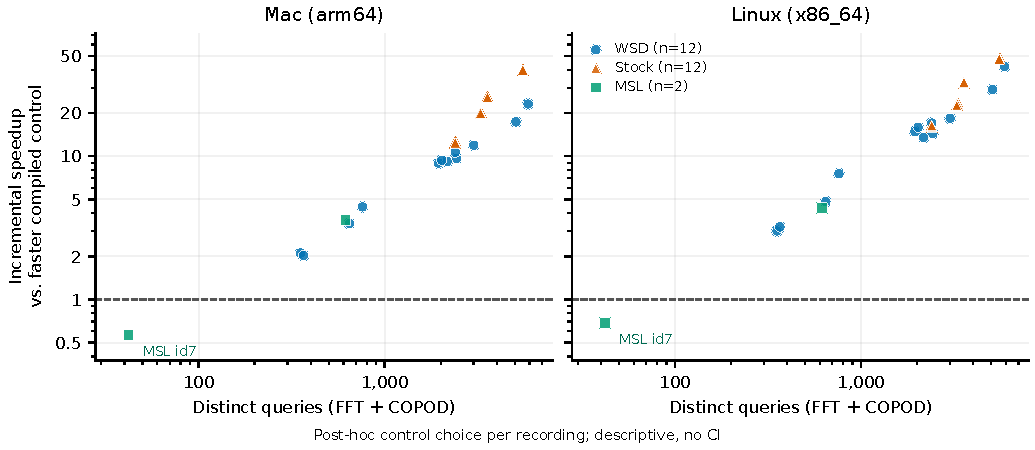
\includegraphics[width=.94\textwidth]{../artifacts/pvldb-research-20261024/strengthening/figures/interval-control-two-host-v1/interval-control-query-regime.pdf}
\caption{Post-hoc descriptive query-regime view of the supplemental study.
Each point is one recording, equally weighting its 12 semantic log ratios.
The denominator is incremental evaluation; the numerator selects the faster
geometric aggregate of raster and interval for that recording. This is a
descriptive lower envelope of measured controls, not a deployable selector or
a prespecified confidence interval. MSL id7 loses on both hosts. Distinct
query counts sum the two public detector profiles.}
\label{fig:query-regime}
\end{figure*}

The native conventional-control ablation retains complete three-metric
read-to-write semantics. At all observed queries, combined interval/bucket
ratios are 3.034 [2.990,3.075] on Mac and 3.190 [3.166,3.224] on Linux.
The faster combined raster control gives 2.732 [2.656,2.812] and
2.756 [2.742,2.773], respectively. At default sampling, raster/bucket is only
1.026 [.998,1.049] and 1.016 [.997,1.033]. Thus the exhaustive-workflow gain
survives the additional control on both hosts, while neither host supports a
default combined-workflow gain over raster. These compiled-only trials add no
public-reference coverage to the earlier study.
\begin{table*}[t]\centering\small
\begin{tabular}{llrrrrr}\toprule
Host & Queries & Raster s & Interval s & Bucket s & Raster/bucket & Interval/bucket\\\midrule
Apple & Nominal 50 & 1.0686 & 1.0991 & 1.0429 & 1.026 [0.998,1.049] & 1.043 [1.016,1.067]\\
Apple & All observed & 2.9474 & 3.2754 & 1.0726 & 2.732 [2.656,2.812] & 3.034 [2.990,3.075]\\
Linux & Nominal 50 & 1.4617 & 1.4880 & 1.4381 & 1.016 [0.997,1.033] & 1.034 [1.015,1.047]\\
Linux & All observed & 4.1126 & 4.7551 & 1.4990 & 2.756 [2.742,2.773] & 3.190 [3.166,3.224]\\
\bottomrule\end{tabular}
\caption{Combined native TimeEval workflows in the separately frozen conventional-control study. Each row evaluates all 52 profiles and all three metrics from CSV read to result write/close. Absolute times are medians of six runs; paired ratios and conditional intervals are independently reconstructed from matched orders. These compiled-only runs supply no additional public-reference coverage.}\label{tab:native-control}
\end{table*}


Across all four original/supplemental Apple/Linux executions, the combined
exhaustive raster/bucket ratio spans 1.932--2.756; results are not pooled.
The two Linux runs have identical hashes for all 52 score profiles and the
shared sources, but their recorded OpenBLAS dispatch architectures differ
(Cooperlake versus SkylakeX). The supplemental combined raster median is
35.2\% higher and bucket median 4.3\% lower than in the original run. These
descriptive differences do not identify a causal CPU or load effect. The
narrow paired-order intervals are conditional within each run and do not
cover this between-run variability.

The same tables give a descriptive cost--fidelity observation, rather than a
same-output speed ratio. Moving from the native nominal default to all observed
queries increases query count from 2,776 to 71,749/71,750 on Mac/Linux, while
the incremental combined workflow's median changes from 1.043 to 1.073 seconds
and from 1.438 to 1.499 seconds. This workload can therefore obtain the complete
native query close to its sampled workflow cost. These are warm-workflow
medians under different query contracts, not paired timing intervals or evidence
of a practically important detector-selection improvement.

The per-collection native results retain practical counterexamples. At default
sampling, Linux MSL favors raster (.981 [.973,.988] raster/bucket), while
Stock's .997 [.967,1.018] interval crosses one. At all observed queries,
interval/bucket on Linux is 1.256 [1.090,1.643] for MSL,
4.649 [4.632,4.666] for Stock and 1.897 [1.849,1.932] for WSD.
The conventional-control ordering for exhaustive WSD changes across hosts:
raster/interval is 1.073 on Mac but .961 on Linux. Reporting only the
slower conventional implementation would overstate the joint-state increment.


\section{Related work and novelty boundary}
The original VUS paper and its effective/efficient extension are the closest
database metric antecedents~\cite{paparrizos2022,boniol2025}. Our formulas
preserve their dynamic target. Sylligardos~\cite{sylligardos2025}, Klein and
Benchopt establish that fast exact evaluation and support cumsums are not new
objectives. The source audit distinguishes current definitions before forming
speed ratios. Tatbul~\cite{tatbul2018} already defines positional weights,
cardinality penalties and closed-form per-overlap evaluation. TimeSeAD already
enumerates observed thresholds, and TimeEval already offers weighted PR curves.
Classical component trees maintain connected level sets and attributes;
linear-time one-dimensional construction predates this work~\cite{najman2006,menotti2007}.
Naegel and Passat~\cite{naegel2014} also incrementally compute component
attributes relative to a fixed binary segmentation target. Label conditioning
itself is therefore established.
Ranefall and W{\"a}hlby already derive per-threshold object precision/recall
from component-size attributes~\cite{ranefall2016}. Their true-positive pixels
are defined by a size interval and their recall denominator by the maximum
such count, rather than fixed labeled anomaly intervals. These constructions
supply related threshold/attribute frameworks. Our additional state must
handle label intersections, fragmentation, and moving weight normalization.
The additional identity maintains \emph{joint label-conditioned overlap and
fragmentation aggregates}, including moving precision weights, across a
trajectory. It is not a new component tree or a new weighting scheme.

The 2024--2026 comparison also includes distinct nearby research questions.
PATE~\cite{ghorbani2024pateproximityawaretimeseries} introduces proximity-aware
evaluation, while we optimize existing targets. TSB-AD~\cite{tsbad} and
TAB~\cite{qiu2025tabunifiedbenchmarkingtime} address benchmark reliability and
unification; ESA~\cite{esa2024} contributes telemetry benchmark conditions.
These motivate reusable evaluation operators rather than establish our state
representation. TSB-AutoAD~\cite{liu2025autoad} and
RAMSAD~\cite{panourgias2026retrievaltrainingsimilaritysearchbased} study selection,
ensembling or retrieval of detector profiles; we make no superior unlabeled
selection claim. mTSBench~\cite{mtsbench} covers a broader multivariate workload,
and the one-liner foundation-model analysis~\cite{zhu2026} studies detection
pipelines rather than incremental metric state.

Formal analysis and LARM/ALARM~\cite{wagner2025formallyexploringtimeseriesanomaly}
examine metric axioms and exclude score-based VUS from their formal scope.
Their properties do not prove this computational identity. CCE offers a
different linear-time metric~\cite{zhong2025cceconfidenceconsistencyevaluationtime};
its native runtime is not an equal-output baseline. A problem-oriented
taxonomy~\cite{yang2026problemorientedtaxonomyevaluationmetrics} and adversarial
reporting analysis~\cite{lyu2026didactuallyfixit} address suitability and
reporting choices. Rank changes themselves are not a new discovery. Our
bounded literature/source search supports the narrower local-state
contribution, not universal precedence over every unpublished implementation.

\section{Reproducibility and limits}
Raw archives and members, decoded arrays, generated scores, source revisions,
protocols and outputs are SHA-256 bound. The primary interval-control and
compiled-consumer results are produced from fresh raw data and public sources with:
\begin{flushleft}\small\ttfamily
python experiments/reproduce\_interval\_control.py\\
\hspace*{1em}--output /tmp/interval-control-replica
\end{flushleft}
The destination must be new; dependencies and observed versions are supplied.
This command fits public profiles, verifies TimeEval loaders, executes both
studies and reconstructs primary tables. The guide supplies separate saved-record
commands for exploratory raster intervals. Original weighted/public-consumer,
five-process and earlier VUS/range reproductions respectively use
\texttt{reproduce\_strengthening.py},
\texttt{reproduce\_affinity\_blocks\_v2.py --run}, and
\texttt{reproduce\_range\_sweep.py --include-vus}, each with a new destination.
Supplementary studies retain separate protocols; TeX compilation is distinct
from numerical reproduction. New raw datasets and score vectors remain local
because redistribution terms are unconfirmed. Acquisition instructions,
identifiers, digests, metric curves and result CSVs are public.

Mathematical claims assume unit-cost exact metric arithmetic. Binary64
experiments give empirical parity, not an all-input rounding certificate.
Canonical integer moments have an explicit size bound; arbitrary polynomial
weights are theorem-only. Native TimeEval integration covers its declared
flat/cardinality-one contract, not every callback option. Low query counts can
favor raster scans, dense VUS support can remove compression gains, and
shared-label batching can increase memory. Warm stored-profile workloads do
not measure detector training, cold compilation or storage durability. Sources
and regenerated scores differ across recorded environments, and repeated
recordings or timing orders are not independent domains. These limits define
where the exact operator acceleration is supported.

\paragraph{Tool assistance.}
AI-assisted tools, including OpenAI Codex, were used for literature search,
mathematical and software development, experiment orchestration, independent
implementation checks, and drafting. The artifact records the validation
procedures and source/result provenance. The sole human author is responsible
for the work; automated audits and simulated reviews are not external peer
review.

\section{Conclusion}
Dynamic VUS and weighted range metrics admit different local sufficient
statistics. Complete ties and predecessor rectangles preserve VUS integrals;
coupled overlap and fragmentation updates preserve weighted range trajectories.
Compilation-matched controls, separate public-detector workloads and native
consumers establish the exact operators' measured operating range and expose
their low-query limits.
